\documentclass{beamer}
\usetheme{Boadilla}
\usepackage{tikz}
 \usepackage[english]{babel}
 \usepackage{amsmath}
 \usepackage{amssymb}
 \usepackage{amsthm}
 \usepackage{animate}
 \usepackage{mathtools} 
 \usepackage[utf8]{inputenc}
 \usepackage{dsfont}
 \usetikzlibrary{patterns}
 \usepackage{mathrsfs}
 \usepackage{bbold}
\usetikzlibrary{mindmap,trees,shadows}
\usepackage{caption}
\usepackage{tabularx}
\usepackage{booktabs}
\usepackage{apacite}
\usepackage{listings}
\captionsetup[figure]{font=scriptsize}
\newcommand{\MYhref}[3][blue]{\href{#2}{\color{#1}{#3}}}%
\usepackage{hyperref} 
            \hypersetup{backref=true,       
                    pagebackref=true,               
                    hyperindex=true,                
                    colorlinks=true,                
                    breaklinks=true,                
                    urlcolor= blue,                
                    linkcolor= blue,                
                    bookmarks=true,                 
                    bookmarksopen=false,
                    citecolor=blue,
                    linkcolor=blue,
                    filecolor=blue,
                    citecolor=blue,
                    linkbordercolor=blue
}

\definecolor{background}{RGB}{39, 40, 34}
\definecolor{string}{RGB}{230, 219, 116}
\definecolor{comment}{RGB}{117, 113, 94}
\definecolor{normal}{RGB}{248, 248, 242}
\definecolor{identifier}{RGB}{166, 226, 46}

\lstset{
  language = SQL,  % choose the language of the code
  linewidth = 12cm,
  numbers = left, % where to put the line-numbers
  stepnumber=1,  % the step between two line-numbers.
  numbersep=5pt, % how far the line-numbers are from the code
  numberstyle=\tiny\color{black}\ttfamily,
  backgroundcolor=\color{background}, % choose the background color. You must add \usepackage{color}
  showspaces=false, % show spaces adding particular underscores
  showstringspaces=false,             % underline spaces within strings
  showtabs=false, % show tabs within strings adding particular underscores
  tabsize=4,                          % sets default tabsize to 2 spaces
  captionpos=b,                       % sets the caption-position to bottom
  breaklines=true,                    % sets automatic line breaking
  breakatwhitespace=true, % sets if automatic breaks should only happen at whitespace
  title=\lstname,  % show the filename of files included with \lstinputlisting;
  basicstyle=\color{normal}\ttfamily,     % sets font style for the code
  keywordstyle=\color{magenta}\ttfamily,  % sets color for keywords
  stringstyle=\color{string}\ttfamily,    % sets color for strings
  commentstyle=\color{comment}\ttfamily,  % sets color for comments
  emph={format_string, eff_ana_bf, permute, eff_ana_btr},
  emphstyle=\color{identifier}\ttfamily,
  belowskip=-0.5cm
}

\newcommand{\pic}[1]{%
    \includegraphics[width=4cm]{#1}
}

\title[High Dimensional Models] % (optional, only for long titles)
{High Dimensional Models}
\subtitle{Time-Varying Graphical Lasso}
\author[Andrew Boomer \& Jacob Pichelmann] % (optional, for multiple authors)
{Andrew Boomer \& Jacob Pichelmann}
\institute []
{Toulouse School of Economics \\ M2 EEE}


\usepackage{graphicx}
\usepackage{grffile}

\date{\today}

\graphicspath{
    {.} % document root dir
    {./Output/}
    {./Report/}
}

\begin{document}


\frame{\titlepage}

\begin{frame}{Network Theory in Practice \cite{page1999pagerank}}
	\begin{itemize}
		\item The Google search algorithm, PageRank, is based on network theory, and is an extension of a measure of network
        importance called eigenvector centrality.
        This measure assigns higher importance to nodes that are connected to other highly connected nodes.
        Search results are sorted according to this network importance vector.
	\end{itemize}

        \begin{figure}
       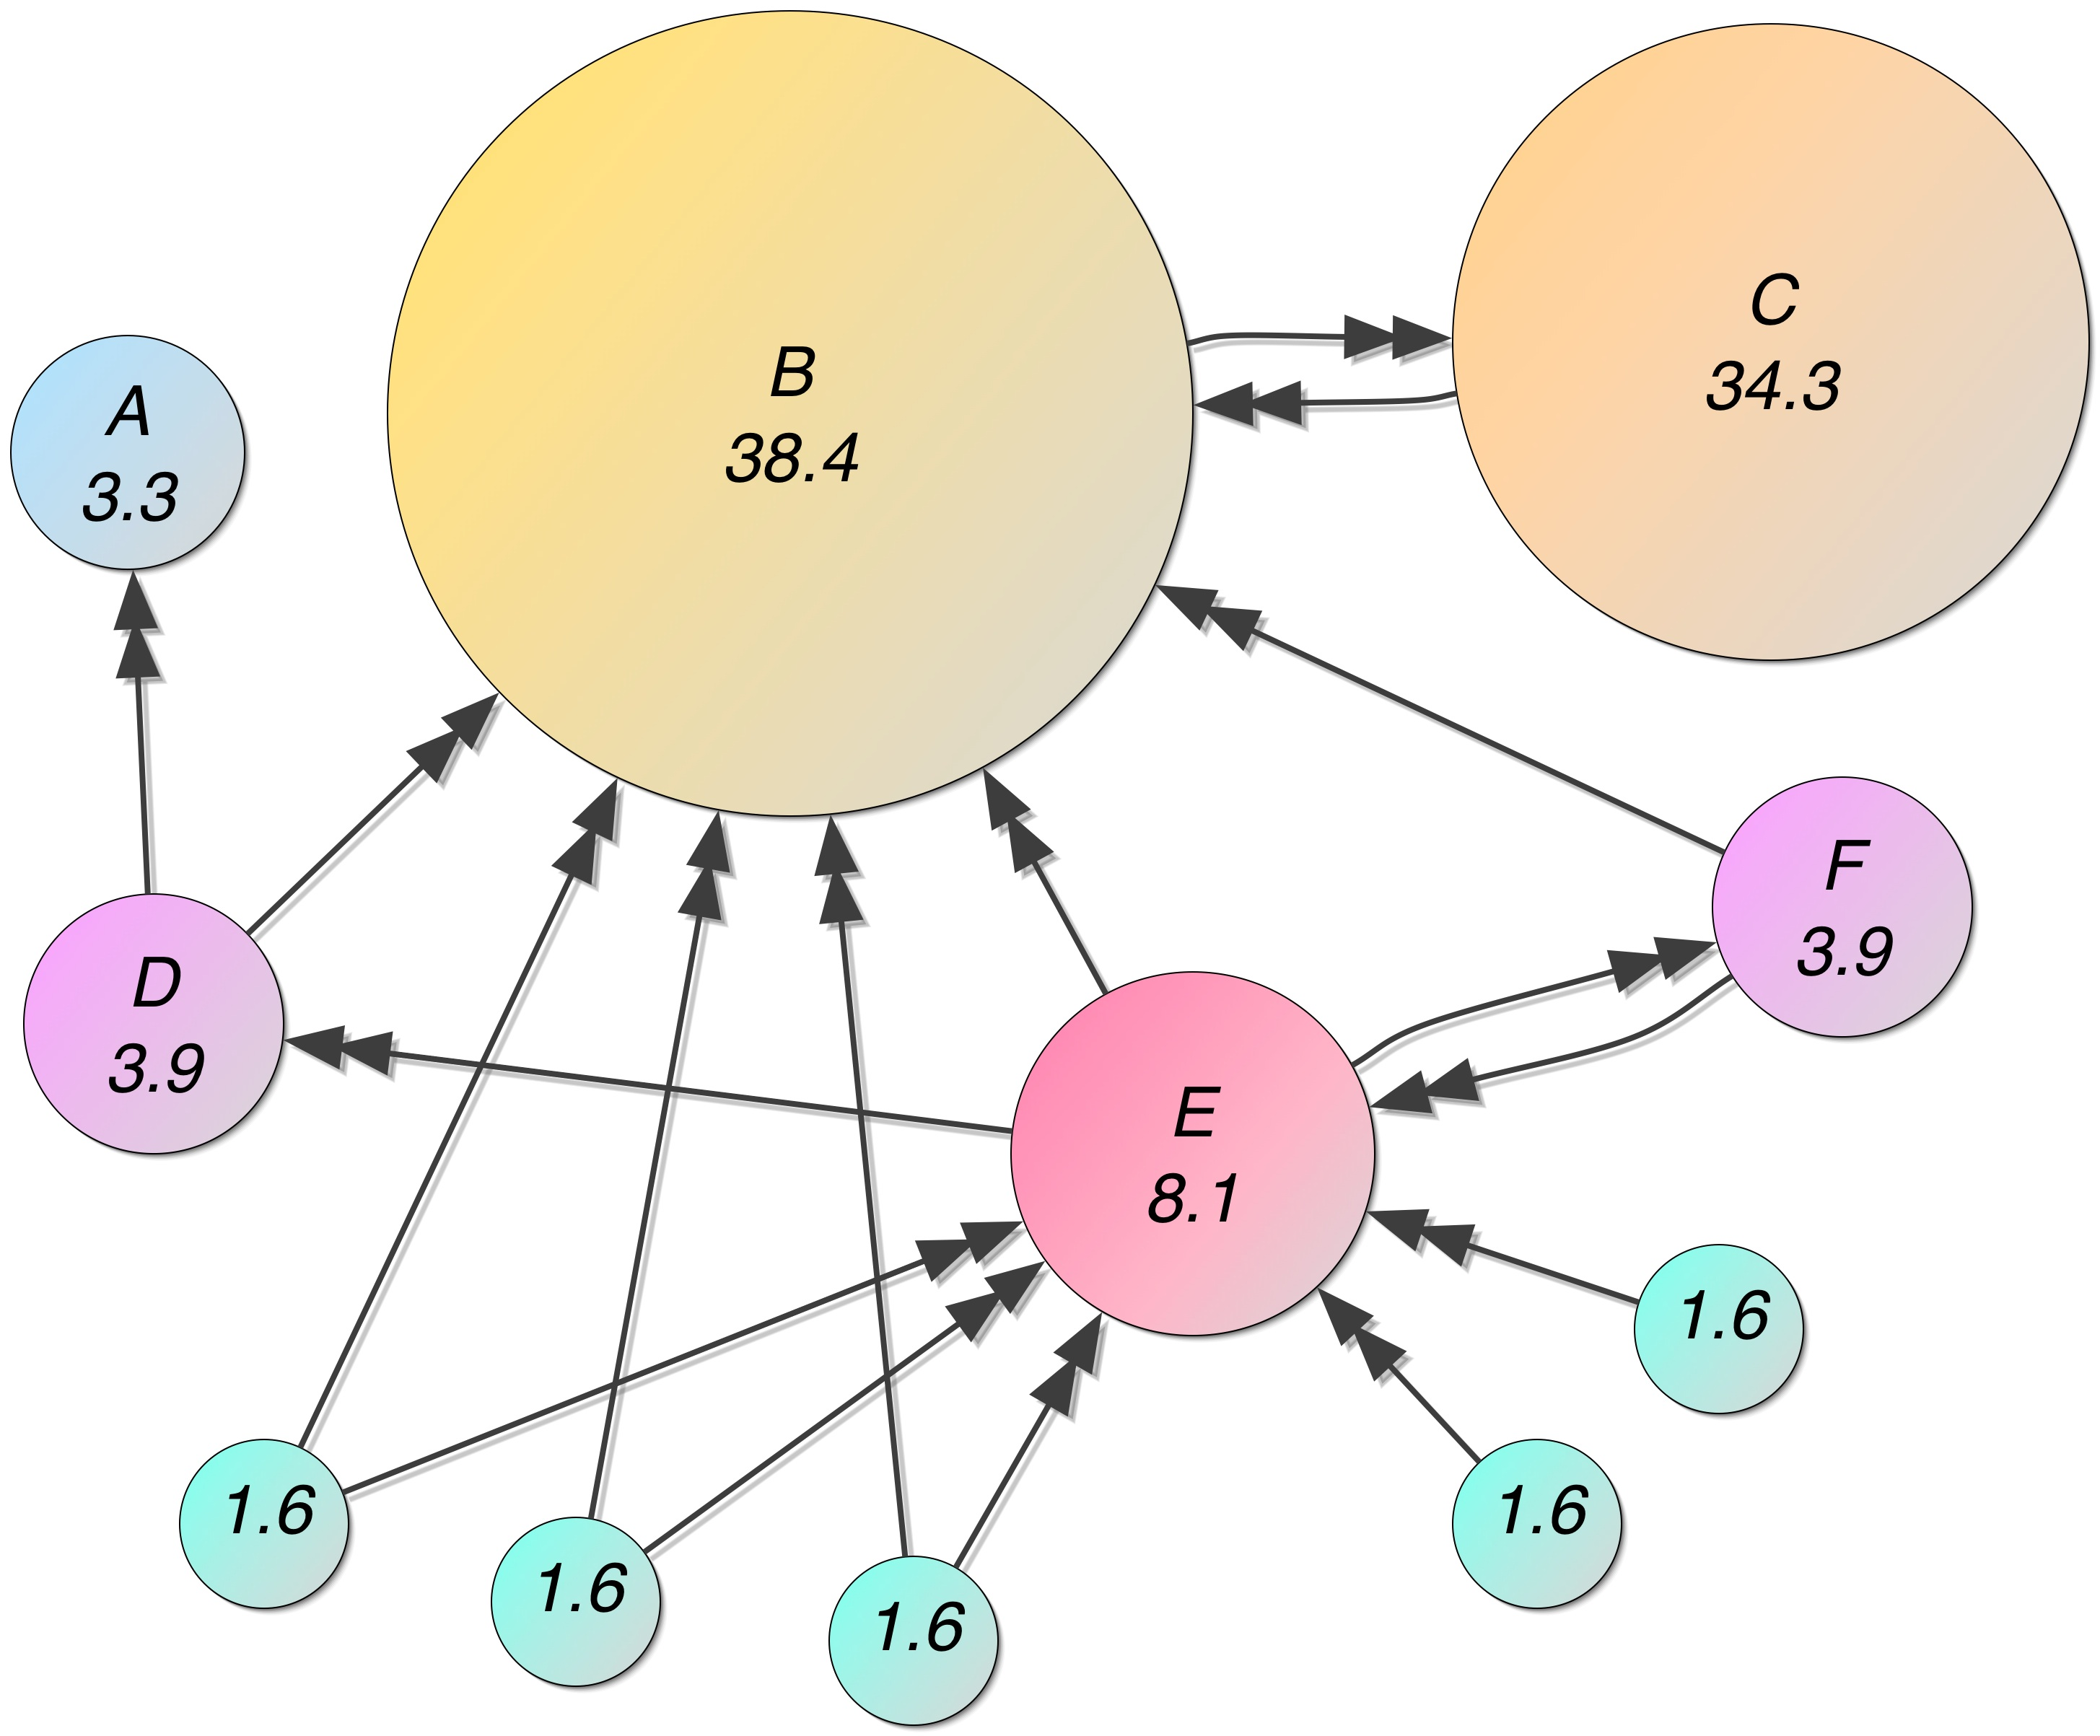
\includegraphics[width=4cm]{PageRankExample}
       \caption{Google Page Rank}
       % \source{}
       \label{fig:PageRank}
  \end{figure}
\end{frame}
    
%\begin{frame}{Introduction to Graphs}
%    \begin{itemize}
%        \item A graph is represented by a set of vertices $V = \{1, 2, \dotsb, p\}$ and by a set of edges $E \subset V x V$
%        \item A graph is undirected when there is no distinction between the edge $(s, t)$ and $(t, s) \quad \forall \ s, t \in E$
%        \item Graphs can also be thought of in terms of Markov chains, and some of the properties and representations of Markov Chains apply to graphs as well
%        \item For example, the edge set of a graph can be represented as a Markov transition matrix.
%        \item For an edge set $E \subset (a, b) x (a, b)$ the matrix would be:
%        \[\begin{bmatrix} W_{(a, a)} & W_{(a, b)} \\
%           W_{(b, a)} & W_{(b, b)} \end{bmatrix}\]
%    \end{itemize}
%\end{frame}

\begin{frame}{Introduction to Graphical Models}
    \footnotesize
  \begin{itemize}
      \item A graph is represented by a set of vertices $V = \{1, 2, \dotsb, p\}$ and by a set of edges $E \subset V x V$
      \item A graph is undirected when there is no distinction between the edge $(s, t)$ and $(t, s) \quad \forall \ s, t \in E$
    \item This graphical representation can be extended to a high dimensional set of random variables $X_{s}$.
    \item In this example, $s$ corresponds to a single vertex with the whole vertex set $V$ of the total graph.
    The connections between each vertex in the Markov transition matrix representation quantify the relationship between this random variables.
  \end{itemize}
  \begin{figure}
  \begin{minipage}{0.4\textwidth}
      The two visualizations in Figure~\ref{fig:IntroPic} are equivalent, where white spaces indicate no relationship, and grey spaces indicate a 1-to-1 relationship.
  \end{minipage}%
  \begin{minipage}{0.6\textwidth}
    \begin{figure}
       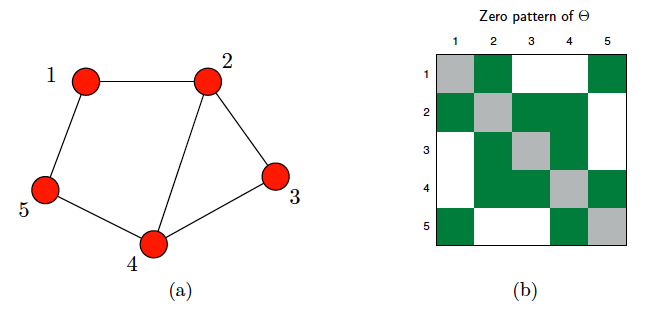
\includegraphics[width=6cm]{IntroGraphMat.png}
       \caption{Graph and Sparsity Matrix}
       \label{fig:IntroPic}
  \end{figure} 
  \end{minipage}
  \end{figure}
\end{frame}


\begin{frame}{Gaussian Graphical Models}
  \begin{itemize}
    \item For a gaussian graphical model, we start from a gaussian distribution with dimension equal to the number of vertices $X \sim \mathcal{N}(\mu, \Sigma)$
    \item The sparsity matrix in the slide above, for a gaussian graphical model, is given by $\Theta = \Sigma^{-1}$, and is also known as the precision matrix. The goal of a gaussian graphical model is to solve for $\Theta$.
    \item The gaussian distribution can be rewritten in terms of a maximum likelihood problem to solve for $\hat{\Theta}_{MLE}$, where $S$ is the empirical covariance matrix, rearranged and simplified to:
    \[\mathcal{L}(\Theta; X) = log \ det \ \Theta - trace(S \Theta)\]
    \item This MLE problem converges to the true precision matrix when $N \xrightarrow{} \infty$.
  \end{itemize}
    % talk about interpretability!
\end{frame}

\begin{frame}{Graphical LASSO}
  \begin{itemize}
      \item The MLE problem is \textbf{not feasible if $p > N$}, where $p$ is the number of dimensions.
    \item As with a LASSO in the context of a linear regression, adding a \textbf{regularization term can solve the issue} of a non-full rank matrix.
    \item Additionally, the LASSO term induces low-importance terms to zero.
      Weak edge connections in the precision matrix will go to zero, increasing the sparsity of the resulting solution.
    Increased sparsity aids in interpretability by filtering out noisy relationships, and can be used even when $N$ is close to $p$.
    \item The graphical lasso estimator is the $\hat{\Theta}$ such that:
\begin{align*}
    \hat{\Theta}=\operatorname{argmin}_{\Theta \geq 0}\left(\operatorname{tr}(S \Theta)-\log \operatorname{det}(\Theta)+\lambda \sum_{j \neq k}\left|\Theta_{j k}\right|\right)
\end{align*}
  \end{itemize}
\end{frame}

\begin{frame}{$\lambda$ in the Context of Networks}
	\begin{itemize}
		\item The penalty parameter determines the structure of the network.
        \item Typical methods can be applied, e.g. cross validation
	\end{itemize}
    \begin{figure}
   \centering
\begin{tabular}{cc}
    $\lambda = 0.05$ & $\lambda = 0.005$ \\
    \pic{NetworkGraph_Alpha0.05_Layoutcircular.png} &  \pic{NetworkGraph_Alpha0.005_Layoutcircular.png} \\
\end{tabular}
\caption{Tuning $\lambda$, own calculations based on data from \cite{hallac2017network}}
   % how to choose alpha?
\label{static_lasso}
\end{figure}
    \end{frame}

\begin{frame}{Challenge: The Network Structure Can Change Over Time}
    In many real world settings (e.g. financial markets) the structure of the complex system changes over time.
    % Intersecting time series analysis and network science allows detecting anomalies, spotting trends and forecasting future behavior.
    \begin{figure}
       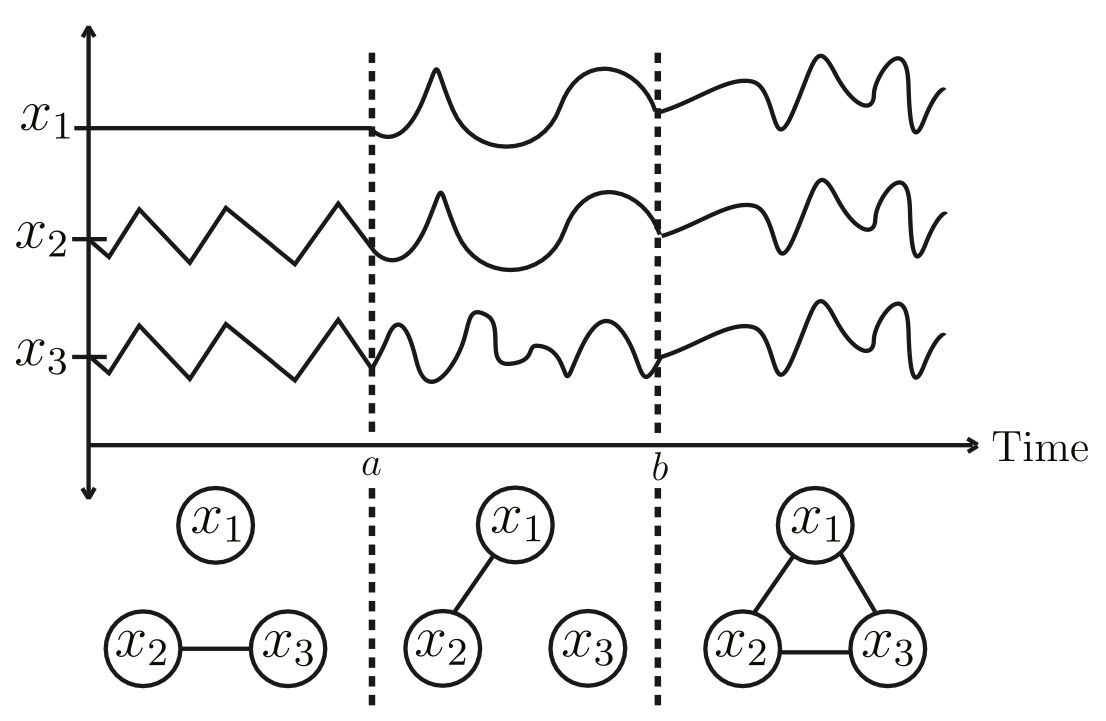
\includegraphics[width=6cm]{network_evolution}
       \caption{}
       % \source{\cite(hallac2017network)}
       \label{fig:network_evolution}
  \end{figure}
\end{frame}

\begin{frame}{Solution: Optimization on a Chain Graph (TVGL)}
    \begin{figure}
       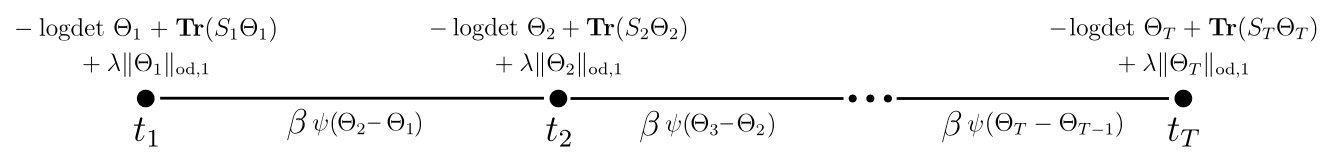
\includegraphics[width=12cm]{chain_graph.png}
       \caption{\cite{hallac2017network}}
       % \source{\cite{hallac2017network}}
       % how to choose beta?
       \label{fig:chain_graph}
  \end{figure}
    The optimization problem becomes
    \begin{align*}
        \underset{\Theta \in \mathrm{S}_{++}^{p}}{\operatorname{minimize}} \quad \sum_{i=1}^{T} \operatorname{Tr}(S_{i} \Theta_{i}) -\log \operatorname{det} \Theta_{i} + \lambda\left\|\Theta_{i}\right\|_{\mathrm{od}, 1}+\beta \sum_{i=2}^{T} \psi\left(\Theta_{i}-\Theta_{i-1}\right)
    \end{align*}
    where $\beta$ determines how strongly correlated neighboring covariance estimations should be.
    A small $\beta$ will lead to $\Theta$'s which fluctuate from estimate-to-estimate, whereas large $\beta$'s lead to smoother estimates over time.
\end{frame}

\begin{frame}{Choice of $\psi$}
    \begin{itemize}
        \item $\psi$ allows to enforce different behaviors in the evolution of the network structure
        \item Expectations of how the underlying network may change over time can be encoded into $\psi$
    \end{itemize}
    Options:
    \begin{itemize}
        % \item \textbf{A few edges changing at a time} - $\psi(X) = \sum_{i,1}|X_{i,j}|$
        % element-wise l1 penalte encourages neighboring graphs to be identical
        \item \textbf{Global restructuring} - $\psi(X) = \sum_j||[X]_j||_2$
        \item \textbf{Smoothly varying over time} - $\psi(X) = \sum_{i,j}X^2_{i,j}$
        % \item \textbf{Block-wise restructuring} - $\psi(X) = \sum_j\left( max_i|X_{i,j}| \right)$
        \item \textbf{Perturbed node} - $\psi(X)=\min _{V: V+V^{T}=X} \sum_{j}\left\|[V]_{j}\right\|_{2}$
    \end{itemize}
\end{frame}

\begin{frame}{Optimization Algorithm: ADMM}

	\begin{itemize}
		\item The authors use an ADMM (alternating direction method of multipliers) to solve the TVGL optimization problem.
		\item ADMM is an general optimization technique that can be used on any convex optimization problem. 
		\item ADMM has a few main advantages compared to standard gradient descent based methods: (1) Can be applied to nonsmooth functions, (2) Can be distributed across multiple independent machines, (3) It is generally faster.
		\item To put ADMM into context, we show how it can be used to solve a standard LASSO regression
	\end{itemize}
\end{frame}

\begin{frame}{Optimization Algorithm: ADMM}
	The LASSO regression optimization problem is:
\[\hat{\beta}_{\lambda} = \underset{\beta}{argmin} \sum_{i=1}^{N} (Y_{i} - X_{i} \beta)^{2} + \lambda \sum_{j=1}^{p} |\beta|\]
\end{frame}

\begin{frame}{GLASSO vs. TVGL}
\underline{Static LASSO}

\begin{itemize}
  \item Date Range: 13/01/2010 - 19/03/2010
  \item Stock List: Apple, MSFT, AMAZON, Intel, Boeing, Fedex
  \item $\alpha = 0.18$
\end{itemize}

  \begin{figure}
    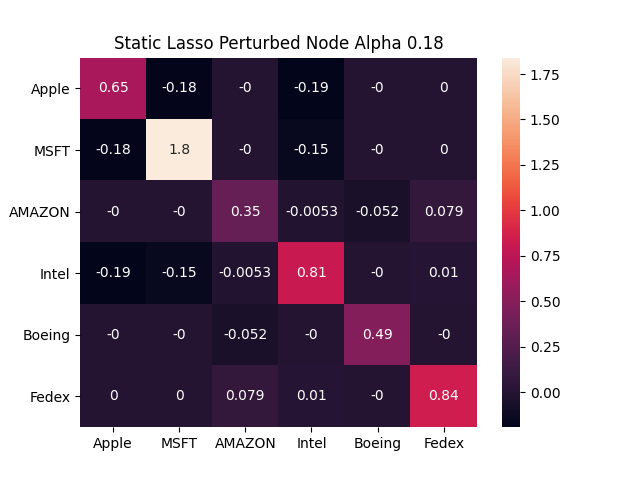
\includegraphics[width=8cm]{Static_Psi5_alpha0.18.png}
    % \caption{}
    \label{fig:static5_0.18}
  \end{figure}

\end{frame}

\begin{frame}{GLASSO vs. TVGL}
\underline{TVGL}
  \begin{columns}
    \begin{column}{0.3\linewidth}
      \begin{itemize}
        \item Date Range, Stock List: Same As Static
        \item ($\alpha$, $\beta$) = ($0.18$, $13$)
        \item $\psi = $ Perturbed Node
      \end{itemize}
    \end{column}
    \begin{column}{0.75\linewidth}
      \animategraphics[loop,controls,height=6.5cm]{1}{PrecMatsPsi5Alpha0.18Beta13}{0}{15}
    \end{column}
  \end{columns}
\end{frame}

\begin{frame}{Importance of $\psi$}
    \begin{itemize}
        \item Choice of $\psi$ relies on knowledge about network behavior
        \item No a priori decision possible
        \item $\psi$ is fixed over time
    \end{itemize}
    We illustrate the importance of the choice of $\psi$ by replicating the author's case studies with different
    penalty functions.
\end{frame}

\begin{frame}{TVGL}
\underline{Sensitivity to Changing Psi}
  \begin{columns}
    \begin{column}{0.3\linewidth}
      \begin{itemize}
        \item Date Range, Stock List: Same As Static
        \item ($\alpha$, $\beta$) = ($0.18$, $13$)
        \item $\psi = $ Smoothly Varying
      \end{itemize}
    \end{column}
    \begin{column}{0.75\linewidth}
      \animategraphics[loop,controls,height=6.5cm]{1}{PrecMatsPsi3Alpha0.18Beta13}{0}{15}
    \end{column}
  \end{columns}
\end{frame}

% \begin{frame}{Extension: Cross Validation for $\psi$}

% \end{frame}

\begin{frame}{Extension: Understanding Network Importance}
    \begin{itemize}
        \item The eigenvector centrality offers a different perspective into the network's dynamic. Though Microsoft obscures the movement somewhat, we can see an uptick in the centrality of Apple.
    \end{itemize}

    \begin{figure}
      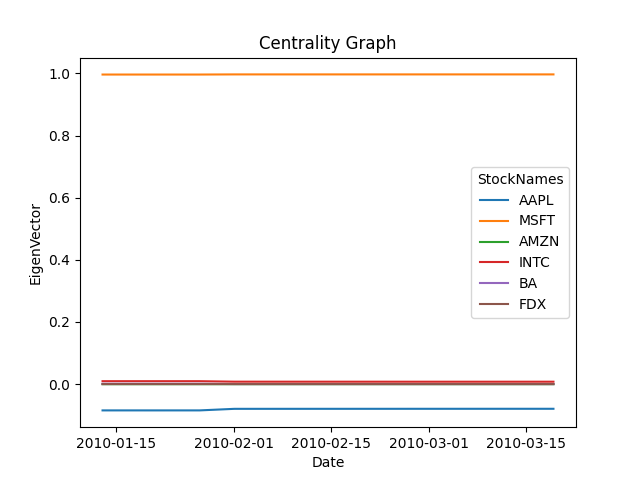
\includegraphics[width=9cm]{EigenVectorCentralityPsi5Alpha0.18Beta13.png}
    \end{figure}
\end{frame}

\begin{frame}{References}
    \nocite{*}
    \bibliographystyle{apacite}
    \bibliography{References}
\end{frame}







\end{document}